\documentclass[tikz,border=0pt]{standalone}
\usepackage[american]{circuitikz}
\usetikzlibrary{arrows.meta,calc,positioning,decorations.pathmorphing,patterns}
\definecolor{zyloTeal}{HTML}{174A5B}
\definecolor{zyloTealTwo}{HTML}{246B7A}
\definecolor{zyloInk}{HTML}{1F2933}
\definecolor{zyloSoft}{HTML}{EAF4F4}
\definecolor{zyloPaper}{HTML}{F8FAFB}
\definecolor{zyloLine}{HTML}{44606B}
\definecolor{zyloOrange}{HTML}{D97706}
\begin{document}
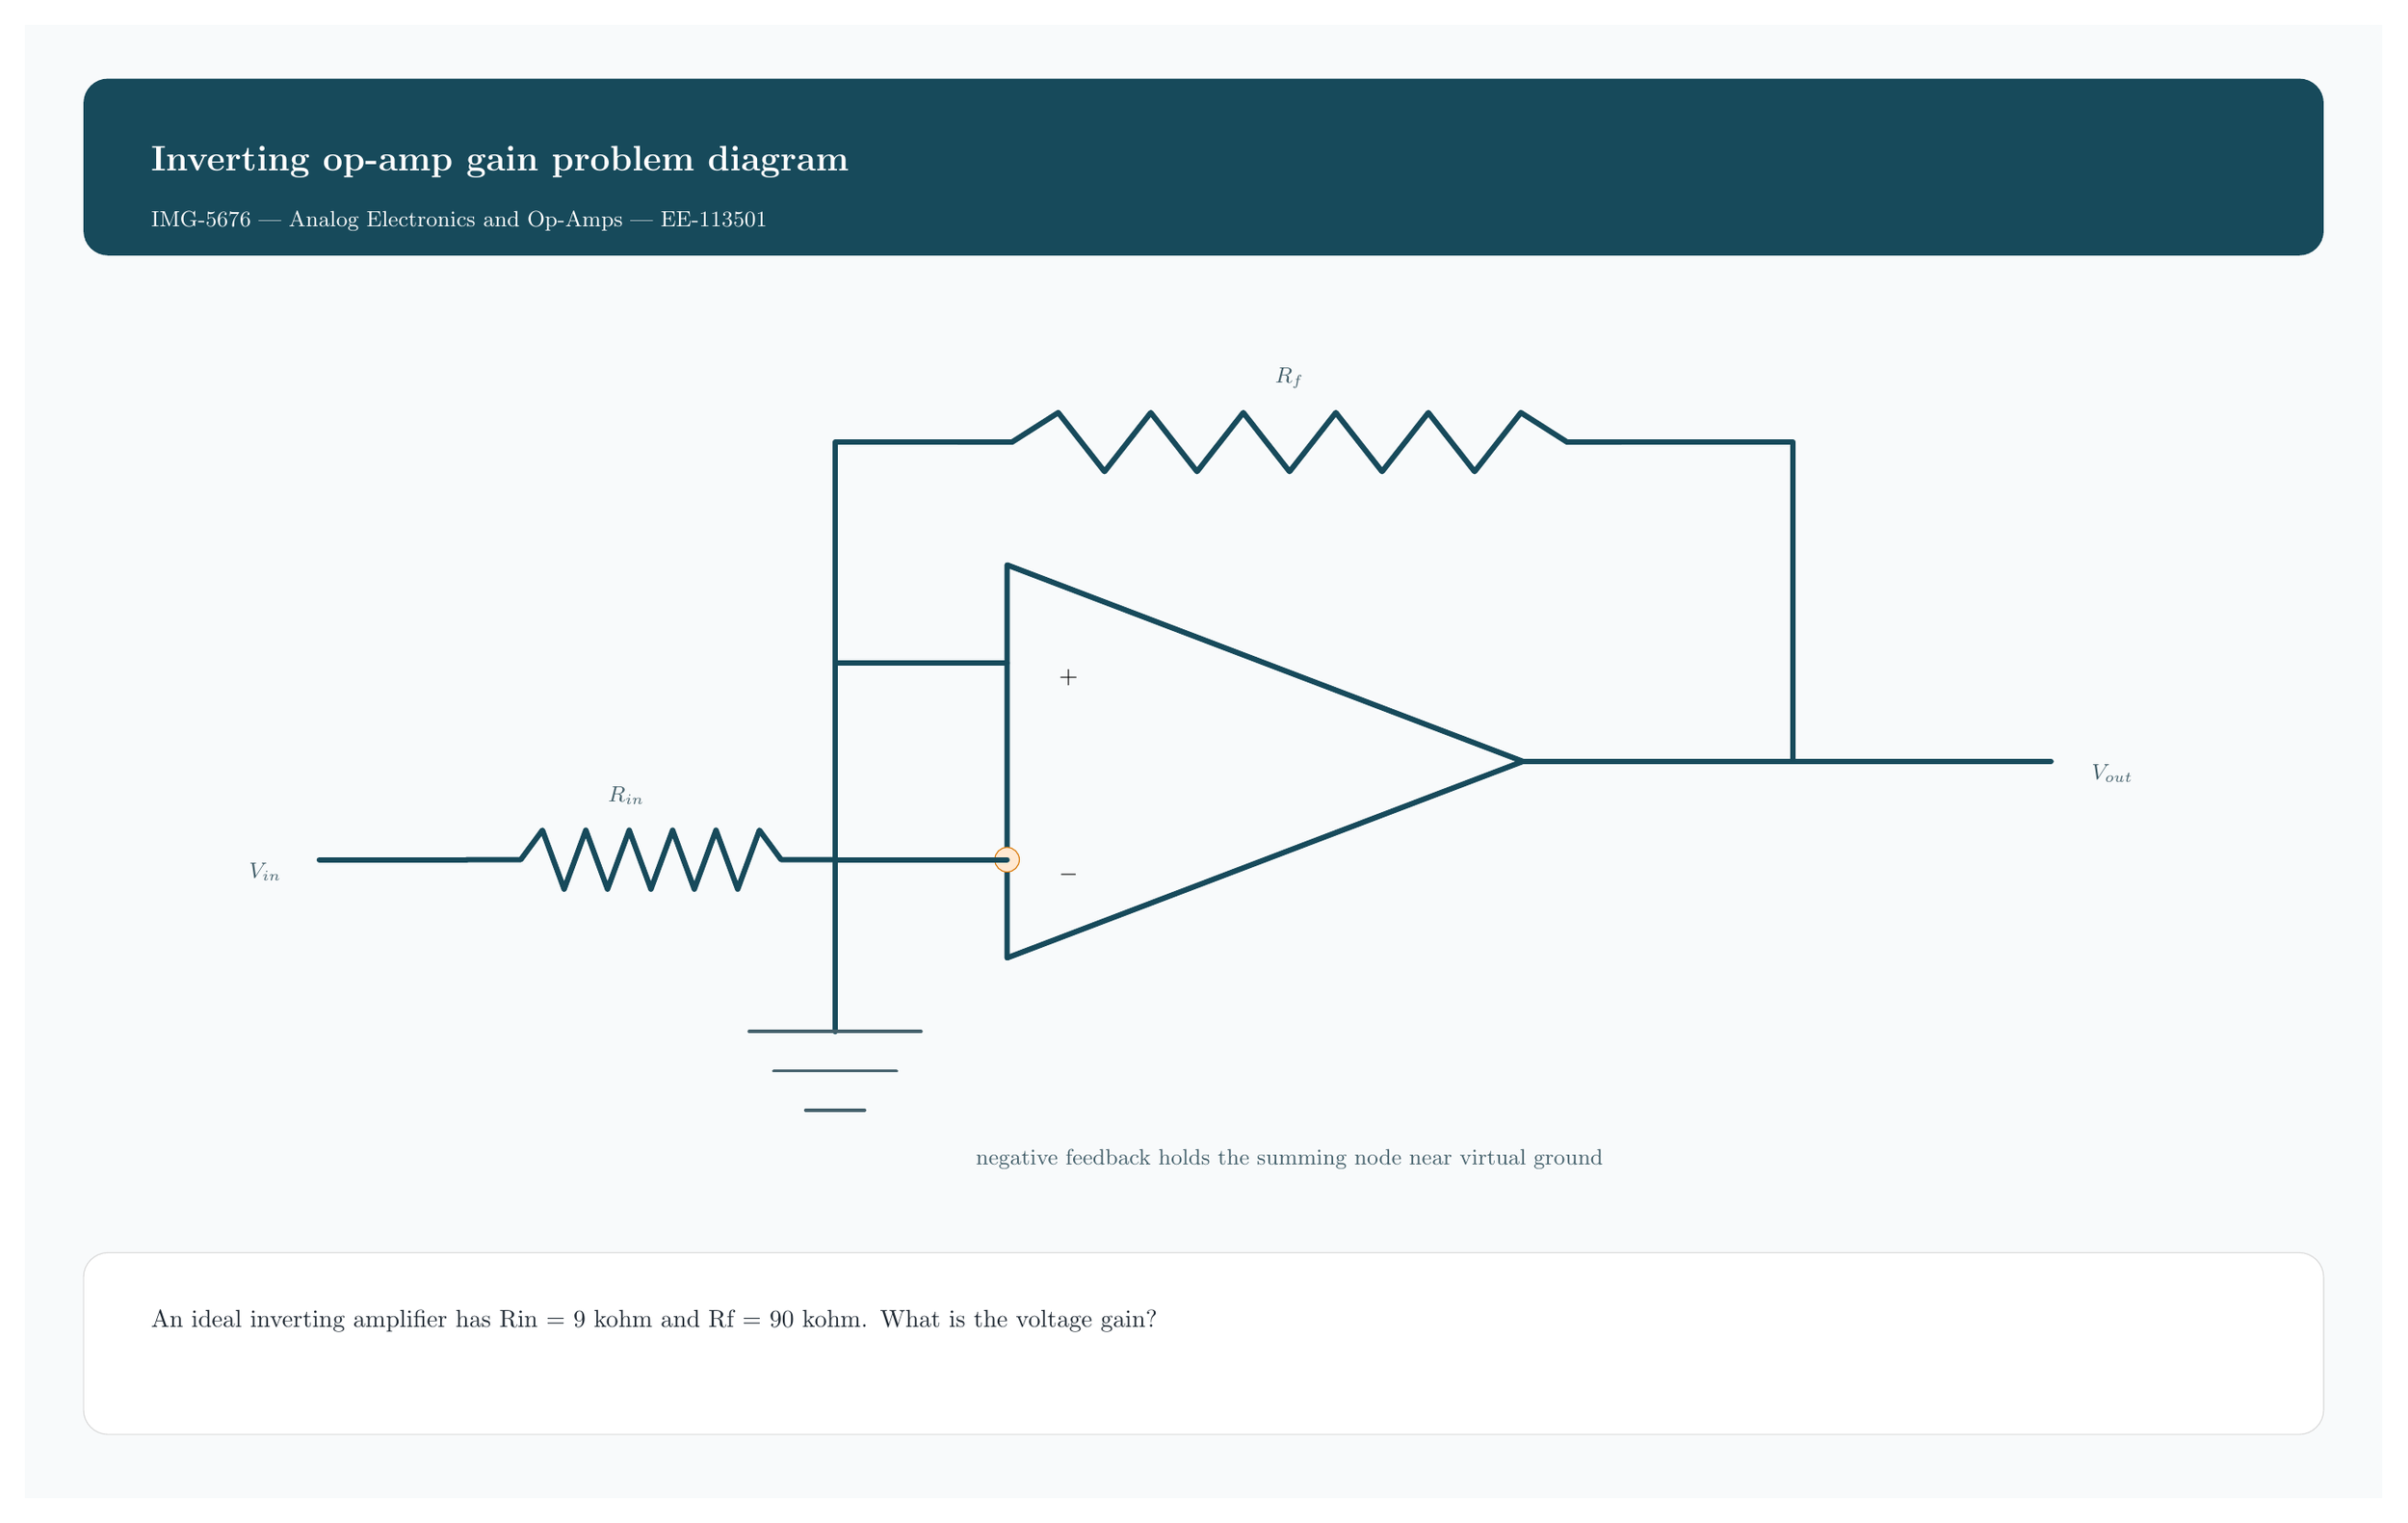
\begin{tikzpicture}[x=1pt,y=-1pt,>=Latex,line cap=round,line join=round]
\path[fill=zyloPaper] (0,0) rectangle (960,600);
\path[fill=zyloTeal,rounded corners=10pt] (24,22) rectangle (936,94);
\node[anchor=west,text=white,font=\bfseries\Large] at (48,56) {Inverting op-amp gain problem diagram};
\node[anchor=west,text=white!82,font=\small] at (48,80) {IMG-5676 | Analog Electronics and Op-Amps | EE-113501};
\tikzset{wire/.style={draw=zyloTeal,line width=2.2pt},thinwire/.style={draw=zyloLine,line width=1.35pt},accent/.style={draw=zyloOrange,line width=2.2pt},box/.style={draw=zyloTealTwo,fill=zyloSoft,line width=1.5pt,rounded corners=8pt}}
\draw[wire] (400,220) -- (400,380) -- (610,300) -- cycle;
\node at (425,266) {$+$}; \node at (425,346) {$-$};
\draw[wire] (120,340) -- (180,340);
\draw[wire] (180,340) -- (202,340) -- (202,340) -- (210.833,328) -- (219.667,352) -- (228.5,328) -- (237.333,352) -- (246.167,328) -- (255,352) -- (263.833,328) -- (272.667,352) -- (281.5,328) -- (290.333,352) -- (299.167,328) -- (308,340) -- (330,340);
\draw[wire] (330,340) -- (400,340); \filldraw[draw=zyloOrange,fill=orange!18] (400,340) circle (5);
\node[font=\small,text=zyloLine] at (245,314) {$R_{in}$}; \node[font=\small,text=zyloLine] at (98,345) {$V_{in}$};
\draw[wire] (610,300) -- (825,300); \node[font=\small,text=zyloLine] at (850,305) {$V_{out}$};
\draw[wire] (400,260) -- (330,260) -- (330,410); \draw[thinwire] (295,410) -- (365,410); \draw[thinwire] (305,426) -- (355,426); \draw[thinwire] (318,442) -- (342,442);
\draw[wire] (400,340) -- (330,340) -- (330,170) -- (380,170);
\draw[wire] (380,170) -- (402,170) -- (402,170) -- (420.833,158) -- (439.667,182) -- (458.5,158) -- (477.333,182) -- (496.167,158) -- (515,182) -- (533.833,158) -- (552.667,182) -- (571.5,158) -- (590.333,182) -- (609.167,158) -- (628,170) -- (650,170);
\draw[wire] (650,170) -- (720,170) -- (720,300); \node[font=\small,text=zyloLine] at (515,144) {$R_f$};
\node[font=\small,text=zyloLine] at (515,462) {negative feedback holds the summing node near virtual ground};
\path[draw=black!15,fill=white,rounded corners=10pt] (24,500) rectangle (936,574);
\node[anchor=west,text width=860pt,align=left,text=zyloInk,font=\normalsize] at (48,528) {An ideal inverting amplifier has Rin = 9 kohm and Rf = 90 kohm. What is the voltage gain?};
\end{tikzpicture}
\end{document}
